% Options for packages loaded elsewhere
\PassOptionsToPackage{unicode}{hyperref}
\PassOptionsToPackage{hyphens}{url}
\PassOptionsToPackage{dvipsnames,svgnames,x11names}{xcolor}
%
\documentclass[
  letterpaper,
  DIV=11,
  numbers=noendperiod]{scrartcl}

\usepackage{amsmath,amssymb}
\usepackage{lmodern}
\usepackage{iftex}
\ifPDFTeX
  \usepackage[T1]{fontenc}
  \usepackage[utf8]{inputenc}
  \usepackage{textcomp} % provide euro and other symbols
\else % if luatex or xetex
  \usepackage{unicode-math}
  \defaultfontfeatures{Scale=MatchLowercase}
  \defaultfontfeatures[\rmfamily]{Ligatures=TeX,Scale=1}
\fi
% Use upquote if available, for straight quotes in verbatim environments
\IfFileExists{upquote.sty}{\usepackage{upquote}}{}
\IfFileExists{microtype.sty}{% use microtype if available
  \usepackage[]{microtype}
  \UseMicrotypeSet[protrusion]{basicmath} % disable protrusion for tt fonts
}{}
\makeatletter
\@ifundefined{KOMAClassName}{% if non-KOMA class
  \IfFileExists{parskip.sty}{%
    \usepackage{parskip}
  }{% else
    \setlength{\parindent}{0pt}
    \setlength{\parskip}{6pt plus 2pt minus 1pt}}
}{% if KOMA class
  \KOMAoptions{parskip=half}}
\makeatother
\usepackage{xcolor}
\setlength{\emergencystretch}{3em} % prevent overfull lines
\setcounter{secnumdepth}{-\maxdimen} % remove section numbering
% Make \paragraph and \subparagraph free-standing
\ifx\paragraph\undefined\else
  \let\oldparagraph\paragraph
  \renewcommand{\paragraph}[1]{\oldparagraph{#1}\mbox{}}
\fi
\ifx\subparagraph\undefined\else
  \let\oldsubparagraph\subparagraph
  \renewcommand{\subparagraph}[1]{\oldsubparagraph{#1}\mbox{}}
\fi

\usepackage{color}
\usepackage{fancyvrb}
\newcommand{\VerbBar}{|}
\newcommand{\VERB}{\Verb[commandchars=\\\{\}]}
\DefineVerbatimEnvironment{Highlighting}{Verbatim}{commandchars=\\\{\}}
% Add ',fontsize=\small' for more characters per line
\usepackage{framed}
\definecolor{shadecolor}{RGB}{241,243,245}
\newenvironment{Shaded}{\begin{snugshade}}{\end{snugshade}}
\newcommand{\AlertTok}[1]{\textcolor[rgb]{0.68,0.00,0.00}{#1}}
\newcommand{\AnnotationTok}[1]{\textcolor[rgb]{0.37,0.37,0.37}{#1}}
\newcommand{\AttributeTok}[1]{\textcolor[rgb]{0.40,0.45,0.13}{#1}}
\newcommand{\BaseNTok}[1]{\textcolor[rgb]{0.68,0.00,0.00}{#1}}
\newcommand{\BuiltInTok}[1]{\textcolor[rgb]{0.00,0.23,0.31}{#1}}
\newcommand{\CharTok}[1]{\textcolor[rgb]{0.13,0.47,0.30}{#1}}
\newcommand{\CommentTok}[1]{\textcolor[rgb]{0.37,0.37,0.37}{#1}}
\newcommand{\CommentVarTok}[1]{\textcolor[rgb]{0.37,0.37,0.37}{\textit{#1}}}
\newcommand{\ConstantTok}[1]{\textcolor[rgb]{0.56,0.35,0.01}{#1}}
\newcommand{\ControlFlowTok}[1]{\textcolor[rgb]{0.00,0.23,0.31}{#1}}
\newcommand{\DataTypeTok}[1]{\textcolor[rgb]{0.68,0.00,0.00}{#1}}
\newcommand{\DecValTok}[1]{\textcolor[rgb]{0.68,0.00,0.00}{#1}}
\newcommand{\DocumentationTok}[1]{\textcolor[rgb]{0.37,0.37,0.37}{\textit{#1}}}
\newcommand{\ErrorTok}[1]{\textcolor[rgb]{0.68,0.00,0.00}{#1}}
\newcommand{\ExtensionTok}[1]{\textcolor[rgb]{0.00,0.23,0.31}{#1}}
\newcommand{\FloatTok}[1]{\textcolor[rgb]{0.68,0.00,0.00}{#1}}
\newcommand{\FunctionTok}[1]{\textcolor[rgb]{0.28,0.35,0.67}{#1}}
\newcommand{\ImportTok}[1]{\textcolor[rgb]{0.00,0.46,0.62}{#1}}
\newcommand{\InformationTok}[1]{\textcolor[rgb]{0.37,0.37,0.37}{#1}}
\newcommand{\KeywordTok}[1]{\textcolor[rgb]{0.00,0.23,0.31}{#1}}
\newcommand{\NormalTok}[1]{\textcolor[rgb]{0.00,0.23,0.31}{#1}}
\newcommand{\OperatorTok}[1]{\textcolor[rgb]{0.37,0.37,0.37}{#1}}
\newcommand{\OtherTok}[1]{\textcolor[rgb]{0.00,0.23,0.31}{#1}}
\newcommand{\PreprocessorTok}[1]{\textcolor[rgb]{0.68,0.00,0.00}{#1}}
\newcommand{\RegionMarkerTok}[1]{\textcolor[rgb]{0.00,0.23,0.31}{#1}}
\newcommand{\SpecialCharTok}[1]{\textcolor[rgb]{0.37,0.37,0.37}{#1}}
\newcommand{\SpecialStringTok}[1]{\textcolor[rgb]{0.13,0.47,0.30}{#1}}
\newcommand{\StringTok}[1]{\textcolor[rgb]{0.13,0.47,0.30}{#1}}
\newcommand{\VariableTok}[1]{\textcolor[rgb]{0.07,0.07,0.07}{#1}}
\newcommand{\VerbatimStringTok}[1]{\textcolor[rgb]{0.13,0.47,0.30}{#1}}
\newcommand{\WarningTok}[1]{\textcolor[rgb]{0.37,0.37,0.37}{\textit{#1}}}

\providecommand{\tightlist}{%
  \setlength{\itemsep}{0pt}\setlength{\parskip}{0pt}}\usepackage{longtable,booktabs,array}
\usepackage{calc} % for calculating minipage widths
% Correct order of tables after \paragraph or \subparagraph
\usepackage{etoolbox}
\makeatletter
\patchcmd\longtable{\par}{\if@noskipsec\mbox{}\fi\par}{}{}
\makeatother
% Allow footnotes in longtable head/foot
\IfFileExists{footnotehyper.sty}{\usepackage{footnotehyper}}{\usepackage{footnote}}
\makesavenoteenv{longtable}
\usepackage{graphicx}
\makeatletter
\def\maxwidth{\ifdim\Gin@nat@width>\linewidth\linewidth\else\Gin@nat@width\fi}
\def\maxheight{\ifdim\Gin@nat@height>\textheight\textheight\else\Gin@nat@height\fi}
\makeatother
% Scale images if necessary, so that they will not overflow the page
% margins by default, and it is still possible to overwrite the defaults
% using explicit options in \includegraphics[width, height, ...]{}
\setkeys{Gin}{width=\maxwidth,height=\maxheight,keepaspectratio}
% Set default figure placement to htbp
\makeatletter
\def\fps@figure{htbp}
\makeatother

\KOMAoption{captions}{tableheading}
\makeatletter
\makeatother
\makeatletter
\makeatother
\makeatletter
\@ifpackageloaded{caption}{}{\usepackage{caption}}
\AtBeginDocument{%
\ifdefined\contentsname
  \renewcommand*\contentsname{Table of contents}
\else
  \newcommand\contentsname{Table of contents}
\fi
\ifdefined\listfigurename
  \renewcommand*\listfigurename{List of Figures}
\else
  \newcommand\listfigurename{List of Figures}
\fi
\ifdefined\listtablename
  \renewcommand*\listtablename{List of Tables}
\else
  \newcommand\listtablename{List of Tables}
\fi
\ifdefined\figurename
  \renewcommand*\figurename{Figure}
\else
  \newcommand\figurename{Figure}
\fi
\ifdefined\tablename
  \renewcommand*\tablename{Table}
\else
  \newcommand\tablename{Table}
\fi
}
\@ifpackageloaded{float}{}{\usepackage{float}}
\floatstyle{ruled}
\@ifundefined{c@chapter}{\newfloat{codelisting}{h}{lop}}{\newfloat{codelisting}{h}{lop}[chapter]}
\floatname{codelisting}{Listing}
\newcommand*\listoflistings{\listof{codelisting}{List of Listings}}
\makeatother
\makeatletter
\@ifpackageloaded{caption}{}{\usepackage{caption}}
\@ifpackageloaded{subcaption}{}{\usepackage{subcaption}}
\makeatother
\makeatletter
\@ifpackageloaded{tcolorbox}{}{\usepackage[many]{tcolorbox}}
\makeatother
\makeatletter
\@ifundefined{shadecolor}{\definecolor{shadecolor}{rgb}{.97, .97, .97}}
\makeatother
\makeatletter
\makeatother
\ifLuaTeX
  \usepackage{selnolig}  % disable illegal ligatures
\fi
\IfFileExists{bookmark.sty}{\usepackage{bookmark}}{\usepackage{hyperref}}
\IfFileExists{xurl.sty}{\usepackage{xurl}}{} % add URL line breaks if available
\urlstyle{same} % disable monospaced font for URLs
\hypersetup{
  pdftitle={Regularización y selección de características},
  pdfauthor={Edmond Géraud},
  colorlinks=true,
  linkcolor={blue},
  filecolor={Maroon},
  citecolor={Blue},
  urlcolor={Blue},
  pdfcreator={LaTeX via pandoc}}

\title{Regularización y selección de características}
\author{Edmond Géraud}
\date{}

\begin{document}
\maketitle
\ifdefined\Shaded\renewenvironment{Shaded}{\begin{tcolorbox}[boxrule=0pt, interior hidden, frame hidden, enhanced, breakable, sharp corners, borderline west={3pt}{0pt}{shadecolor}]}{\end{tcolorbox}}\fi

\hypertarget{selecciuxf3n-de-caracteruxedsticas}{%
\section{Selección de
características}\label{selecciuxf3n-de-caracteruxedsticas}}

La selección de características es una técnica utilizada en aprendizaje
automático para seleccionar un subconjunto de características relevantes
y útiles para la tarea de predicción, con el objetivo de mejorar el
rendimiento del modelo y reducir el riesgo de sobreajuste. En otras
palabras, la selección de características se refiere al proceso de
elegir un conjunto óptimo de características (variables o atributos)
para el modelo predictivo, eliminando las características redundantes o
irrelevantes que pueden afectar negativamente el rendimiento del modelo.

\hypertarget{selecciuxf3n-de-modelos-por-aic}{%
\subsection{Selección de modelos por
AIC}\label{selecciuxf3n-de-modelos-por-aic}}

El criterio de información de Akaike (AIC) es un método para seleccionar
modelos estadísticos entre un conjunto de modelos candidatos. Fue
propuesto por el estadístico japonés Hirotugu Akaike en 1974.

El principio subyacente del AIC es que se prefiere un modelo que tenga
un buen ajuste a los datos, pero que tenga un número mínimo de
parámetros. El AIC combina estas dos medidas al considerar tanto la
bondad de ajuste del modelo como el número de parámetros del modelo.

El AIC se define como la suma del error cuadrático (o alguna otra medida
de error) del modelo y el producto del número de parámetros del modelo y
una constante que depende del número de observaciones. El modelo con el
valor más bajo del AIC se considera el mejor modelo de entre los modelos
candidatos.

El AIC se basa en la idea de que el modelo más probable es aquel que
minimiza la información perdida al modelar los datos, es decir, que
tiene el equilibrio óptimo entre el ajuste y la complejidad del modelo.
El término de penalización del número de parámetros en el AIC evita que
el modelo se sobreajuste a los datos y selecciona el modelo más simple
posible que aún pueda explicar los datos de manera efectiva.

En resumen, el principio subyacente del AIC es encontrar un modelo que
tenga un buen ajuste a los datos, pero que tenga un número mínimo de
parámetros. El AIC se basa en la idea de que el modelo más probable es
aquel que minimiza la información perdida al modelar los datos, y
utiliza una medida combinada de la bondad de ajuste y la complejidad del
modelo para seleccionar el mejor modelo de entre los modelos candidatos.

\[
AIC=2k-2ln(L)
\]

Donde \(k\) es el número de parámetros en el modelo y \(L\) es la
función de verosimilitud máxima del modelo estimada a partir de los
datos.

El AIC se calcula como la suma de dos términos: el primer término, 2k,
es una penalización por el número de parámetros en el modelo, mientras
que el segundo término, \(-2ln(L)\), es proporcional al negativo del
logaritmo de la función de verosimilitud máxima del modelo. El modelo
con el valor más bajo del AIC se considera el mejor modelo de entre los
modelos candidatos.

\hypertarget{muxe9todos-por-reducciuxf3n-de-dimensionalidad}{%
\subsection{Métodos por reducción de
dimensionalidad}\label{muxe9todos-por-reducciuxf3n-de-dimensionalidad}}

\hypertarget{pca-pcr}{%
\subsubsection{PCA-PCR}\label{pca-pcr}}

El PCA (Principal Component Analysis) es una técnica estadística
utilizada para reducir la dimensionalidad de los datos. El objetivo del
PCA es encontrar una combinación lineal de variables predictoras
(conocidas como componentes principales) que expliquen la mayor cantidad
posible de la variación en los datos.

En el PCA, se asume que la variación en los datos se debe a una
combinación de variables predictoras y no a variables aleatorias. Por lo
tanto, el PCA busca identificar las variables predictoras que
contribuyen más a la variación en los datos y combinarlas para formar
nuevas variables o componentes principales.

La primera componente principal se elige de tal manera que tenga la
mayor varianza posible, lo que significa que esta componente principal
explica la mayor cantidad posible de la variación en los datos. Las
componentes siguientes se eligen de tal manera que estén altamente
correlacionadas con las variables predictoras originales, pero no estén
correlacionadas con las componentes principales previamente
seleccionadas.

Una vez que se han identificado las componentes principales, se pueden
utilizar para reducir la dimensionalidad de los datos al proyectar los
datos originales sobre las componentes principales seleccionadas. Esto
se puede hacer eliminando las componentes principales que contribuyen
menos a la variación en los datos y conservando solo las componentes
principales más importantes.

El PCA se utiliza comúnmente en la exploración de datos y el análisis
multivariado, particularmente en los casos en que hay muchas variables
predictoras. También se utiliza en la clasificación y la agrupación de
datos y en la visualización de datos en dos o tres dimensiones.

En resumen, el PCA es una técnica estadística utilizada para reducir la
dimensionalidad de los datos. El PCA busca identificar las variables
predictoras que contribuyen más a la variación en los datos y
combinarlas para formar nuevas variables o componentes principales. Las
componentes principales se pueden utilizar para reducir la
dimensionalidad de los datos proyectando los datos originales sobre las
componentes principales seleccionadas.

El PCR (Principal Component Regression) es un método de regresión que
utiliza el PCA para reducir la dimensionalidad de los datos y luego
realiza la regresión sobre las componentes principales seleccionadas. En
lugar de utilizar todas las variables predictoras originales en la
regresión, el PCR utiliza una combinación lineal de las componentes
principales seleccionadas que mejor explique la variabilidad en la
variable respuesta.

En el PCR, se realizan tres pasos principales. En primer lugar, se
realiza el PCA sobre las variables predictoras para identificar las
componentes principales que explican la mayor cantidad de variación en
los datos. En segundo lugar, se seleccionan un número limitado de
componentes principales que se utilizarán en la regresión. En tercer
lugar, se realiza la regresión utilizando las componentes principales
seleccionadas.

El objetivo del PCR es reducir la dimensionalidad de los datos para
evitar el sobreajuste del modelo y mejorar la precisión de la regresión.
El PCR se utiliza comúnmente en la regresión cuando hay muchas variables
predictoras y es difícil identificar cuáles son las variables más
importantes.

El PCR tiene algunas ventajas en comparación con otros métodos de
regresión, como la regresión lineal múltiple. En particular, el PCR
puede ser útil cuando hay una alta correlación entre las variables
predictoras, lo que puede causar problemas en la regresión lineal
múltiple. Además, el PCR puede mejorar la estabilidad de la regresión al
reducir la dimensionalidad de los datos.

En resumen, el PCR es un método de regresión que utiliza el PCA para
reducir la dimensionalidad de los datos y luego realiza la regresión
sobre las componentes principales seleccionadas. El PCR se utiliza
comúnmente en la regresión

Stop generating

\hypertarget{pls}{%
\subsubsection{PLS}\label{pls}}

El PLS (Partial Least Squares) es un método estadístico de regresión que
busca establecer una relación lineal entre un conjunto de variables
predictoras y una variable respuesta. El objetivo de PLS es encontrar
una representación reducida de las variables predictoras, llamadas
componentes latentes, que expliquen la mayor cantidad posible de
variación en la variable respuesta.

La idea principal del PLS es encontrar una combinación lineal de las
variables predictoras que explique la mayor parte de la variación en la
variable respuesta. Para lograr esto, PLS utiliza una técnica de
descomposición en componentes principales que se enfoca en encontrar una
relación lineal entre las variables predictoras y la variable respuesta.

La técnica de PLS busca encontrar una representación reducida de los
datos de entrada mediante la creación de un conjunto de componentes
latentes. Estos componentes latentes son combinaciones lineales de las
variables predictoras originales que están altamente correlacionadas con
la variable respuesta. Cada componente latente se construye de manera
que tenga la máxima covarianza posible con la variable respuesta y, al
mismo tiempo, esté altamente correlacionado con las variables
predictoras originales.

La técnica de PLS se utiliza comúnmente en el análisis multivariado de
datos, particularmente en la regresión de datos altamente
correlacionados o cuando hay muchas variables predictoras en comparación
con el número de observaciones disponibles. Además, PLS se puede
utilizar para reducir la dimensionalidad de un conjunto de datos para su
posterior análisis, así como para identificar las variables predictoras
más importantes en un modelo de regresión.

\hypertarget{muxe9todos-de-regularizaciuxf3n}{%
\subsection{Métodos de
regularización}\label{muxe9todos-de-regularizaciuxf3n}}

La regularización en los métodos de regresión es una técnica utilizada
para evitar el sobreajuste o la falta de generalización de un modelo de
regresión. El sobreajuste ocurre cuando un modelo se ajusta demasiado
bien a los datos de entrenamiento, lo que puede hacer que sea demasiado
específico y no se generalice bien a nuevos datos. La regularización es
una técnica que impone restricciones al modelo de regresión, con el
objetivo de reducir la complejidad y evitar el sobreajuste.

Existen diferentes tipos de regularización, como la regularización L1
(también conocida como LASSO), la regularización L2 (también conocida
como Ridge) y la regularización Elastic Net, que combina ambas técnicas.
Estas técnicas agregan una penalización a la función de costo del modelo
de regresión, lo que permite controlar la complejidad del modelo y
evitar el sobreajuste.

La regularización es una técnica muy útil en el aprendizaje automático,
especialmente en problemas de regresión donde se trabaja con grandes
conjuntos de datos y se desea obtener modelos que sean generalizables y
no sobreajustados a los datos de entrenamiento.

La regularización L2 agrega una penalización a la función de costo del
modelo de regresión que es proporcional al cuadrado de los coeficientes
del modelo. Esta penalización reduce los coeficientes de las
características menos relevantes, lo que significa que el modelo se
centrará más en las características que son más importantes para la
predicción.

Una vez que se ha entrenado el modelo de regresión con la técnica de
regularización L2, es posible utilizar los coeficientes resultantes para
identificar las características más importantes. Estas características
pueden seleccionarse y utilizarse para entrenar otro modelo, como un
modelo de clasificación, por ejemplo.

Es importante tener en cuenta que la selección de características debe
realizarse con cuidado y que no siempre es adecuado utilizar solo las
características más importantes para entrenar un modelo, ya que pueden
perderse información importante. Por lo tanto, es recomendable realizar
un análisis cuidadoso de las características antes de seleccionar las
más relevantes.

Si el modelo de regresión lineal es el siguiente:

\[
Y=X\beta+\epsilon
\]

La regularización L1 o Lasso intenta minimizar la siguiente ecuación

\[
\text{min } \frac{1}{2n} \sum_{i=1}^{n}(y_i - \beta_0 - \sum_{j=1}^{p}x_{ij}\beta_j)^2 + \lambda\sum_{j=1}^{p}|\beta_j|
\]

La regularización L2 o ridge:

\[
\text{min } \frac{1}{2n} \sum_{i=1}^{n}(y_i - \beta_0 - \sum_{j=1}^{p}x_{ij}\beta_j)^2 + \lambda\sum_{j=1}^{p}\beta_j^2
\]

La elastic net:

\$\$
\[\text{min } \frac{1}{2n} \sum_{i=1}^{n}(y_i - \beta_0 - \sum_{j=1}^{p}x_{ij}\beta_j)^2 + \lambda_1\sum_{j=1}^{p}|\beta_j| + \lambda_2\sum_{j=1}^{p}\beta_j^2
\]

Los métodos de regularización como L1, L2 y Elastic Net no tienen una
solución cerrada o analítica, y generalmente se utilizan métodos
numéricos iterativos para encontrar los coeficientes óptimos del modelo.

Estos métodos iterativos se basan en el principio de minimización del
error cuadrático (o alguna otra medida de error) del modelo, junto con
la función de regularización. Por ejemplo, el algoritmo de descenso de
gradiente puede ser utilizado para optimizar la función objetivo de
regresión con regularización.

Además, es importante ajustar el parámetro de regularización \(\lambda\)
(o \(\lambda_1\) y \(\lambda_2\) en el caso de Elastic Net) para
encontrar un equilibrio adecuado entre el ajuste del modelo y la
regularización. Esto se puede hacer mediante la validación cruzada o
mediante el uso de algoritmos de optimización más avanzados, como la
búsqueda de cuadrícula o la optimización bayesiana.

En resumen, se utilizan métodos iterativos y de optimización para
encontrar la solución óptima en métodos de regularización, lo que hace
que su implementación sea más compleja que en los métodos de regresión
lineal sin regularización.

El método de descenso de gradiente es un algoritmo iterativo de
optimización utilizado para minimizar una función de costo. En el
contexto de los métodos de regresión con regularización, esta función de
costo se define como la suma del error cuadrático (o alguna otra medida
de error) del modelo, junto con la función de regularización.

El algoritmo de descenso de gradiente comienza con un valor inicial de
los coeficientes del modelo, y en cada iteración actualiza los valores
de los coeficientes en la dirección opuesta al gradiente de la función
de costo. La idea es que al actualizar los coeficientes en esta
dirección, se reducirá gradualmente el valor de la función de costo.

El tamaño de los pasos que se dan en cada iteración se controla mediante
un parámetro conocido como la tasa de aprendizaje. Si la tasa de
aprendizaje es demasiado pequeña, el algoritmo puede converger
lentamente, mientras que si es demasiado grande, puede no converger en
absoluto. Por lo tanto, elegir una tasa de aprendizaje adecuada es
importante para el éxito del algoritmo.

El algoritmo de descenso de gradiente puede repetirse hasta que se
alcanza un criterio de convergencia predefinido, como una tolerancia de
error o un número máximo de iteraciones. Una vez que se alcanza la
convergencia, se devuelve el valor óptimo de los coeficientes del
modelo.

\hypertarget{muxe9tricas}{%
\section{Métricas}\label{muxe9tricas}}

Existen varias métricas que se utilizan comúnmente para evaluar la
rendición de los modelos, dependiendo del tipo de problema y del tipo de
modelo utilizado. Aquí te presento algunas de las métricas más comunes:

\begin{itemize}
\item
  Error cuadrático medio (MSE): Esta métrica mide la media de los
  errores al cuadrado entre las predicciones del modelo y los valores
  reales de la variable respuesta. El MSE es muy utilizado en problemas
  de regresión.
\item
  Coeficiente de determinación (R\^{}2): Esta métrica mide la proporción
  de la variabilidad en la variable respuesta que es explicada por el
  modelo. Un valor de R\^{}2 cercano a 1 indica que el modelo explica
  bien la variabilidad en la variable respuesta, mientras que un valor
  cercano a 0 indica que el modelo no es capaz de explicar la
  variabilidad. El R\^{}2 es muy utilizado en problemas de regresión.
\item
  Exactitud (accuracy): Esta métrica mide la proporción de predicciones
  correctas del modelo en relación al total de predicciones. El accuracy
  es muy utilizado en problemas de clasificación.
\item
  Precisión (precision) y recuperación (recall): Estas métricas se
  utilizan comúnmente en problemas de clasificación binaria para evaluar
  la calidad de las predicciones positivas del modelo. La precisión mide
  la proporción de predicciones positivas correctas en relación al total
  de predicciones positivas, mientras que la recuperación mide la
  proporción de instancias positivas que son correctamente clasificadas
  por el modelo.
\item
  F1-score: Esta métrica combina la precisión y la recuperación en una
  única medida que se utiliza comúnmente en problemas de clasificación
  binaria.
\end{itemize}

Cabe destacar que no hay una métrica única que sea la más utilizada para
evaluar la rendición de los modelos, ya que la elección de la métrica
depende del tipo de problema y del tipo de modelo utilizado. En general,
se recomienda utilizar varias métricas para evaluar la rendición de los
modelos y obtener una visión más completa del desempeño del modelo.

\[
\text{MSE} = \frac{1}{n} \sum_{i=1}^{n} (y_i - \hat{y}_i)^2
\]

\[
R^2 = 1 - \frac{\sum_{i=1}^{n} (y_i - \hat{y}i)^2}{\sum{i=1}^{n} (y_i - \bar{y})^2}
\]

\hypertarget{pruxe1ctica}{%
\section{Práctica}\label{pruxe1ctica}}

\textbf{De los datos \texttt{fat} del paquete \texttt{faraway},utiliza
el porcentaje de grasa,\texttt{siri}, como la respuesta, y las otras
variables como independientes, excepto \texttt{brozek} y
\texttt{density}. Quita una observación cada 10 del conjunto de datos
para formar el conjunto de entrenamiento y el de prueba.}

\textbf{Realiza los siguientes modelos:}

\begin{enumerate}
\def\labelenumi{\arabic{enumi}.}
\tightlist
\item
  \textbf{Regresión múltiple lineal}
\item
  \textbf{Regresión múlitple seleccionando variables con AIC}
\item
  \textbf{PCR}
\item
  \textbf{PLS}
\item
  \textbf{Ridge}
\item
  \textbf{LASSO}
\end{enumerate}

\hypertarget{cargamos-libreruxedas-y-carga-de-datos}{%
\subsubsection{Cargamos librerías y carga de
datos}\label{cargamos-libreruxedas-y-carga-de-datos}}

\begin{Shaded}
\begin{Highlighting}[]
\FunctionTok{library}\NormalTok{(faraway)}
\FunctionTok{library}\NormalTok{(ggstatsplot)}
\end{Highlighting}
\end{Shaded}

\begin{verbatim}
You can cite this package as:
     Patil, I. (2021). Visualizations with statistical details: The 'ggstatsplot' approach.
     Journal of Open Source Software, 6(61), 3167, doi:10.21105/joss.03167
\end{verbatim}

\begin{Shaded}
\begin{Highlighting}[]
\FunctionTok{library}\NormalTok{(DescTools)}
\FunctionTok{library}\NormalTok{(corrplot)}
\end{Highlighting}
\end{Shaded}

\begin{verbatim}
corrplot 0.92 loaded
\end{verbatim}

\begin{Shaded}
\begin{Highlighting}[]
\FunctionTok{library}\NormalTok{(leaps)}
\FunctionTok{library}\NormalTok{(pls)}
\end{Highlighting}
\end{Shaded}

\begin{verbatim}

Attaching package: 'pls'
\end{verbatim}

\begin{verbatim}
The following object is masked from 'package:corrplot':

    corrplot
\end{verbatim}

\begin{verbatim}
The following object is masked from 'package:stats':

    loadings
\end{verbatim}

\begin{Shaded}
\begin{Highlighting}[]
\FunctionTok{library}\NormalTok{(MASS)}
\FunctionTok{library}\NormalTok{(glmnet)}
\end{Highlighting}
\end{Shaded}

\begin{verbatim}
Loading required package: Matrix
\end{verbatim}

\begin{verbatim}
Loaded glmnet 4.1-7
\end{verbatim}

\begin{Shaded}
\begin{Highlighting}[]
\NormalTok{datos }\OtherTok{\textless{}{-}}\NormalTok{ fat}
\FunctionTok{str}\NormalTok{(fat)}
\end{Highlighting}
\end{Shaded}

\begin{verbatim}
'data.frame':   252 obs. of  18 variables:
 $ brozek : num  12.6 6.9 24.6 10.9 27.8 20.6 19 12.8 5.1 12 ...
 $ siri   : num  12.3 6.1 25.3 10.4 28.7 20.9 19.2 12.4 4.1 11.7 ...
 $ density: num  1.07 1.09 1.04 1.08 1.03 ...
 $ age    : int  23 22 22 26 24 24 26 25 25 23 ...
 $ weight : num  154 173 154 185 184 ...
 $ height : num  67.8 72.2 66.2 72.2 71.2 ...
 $ adipos : num  23.7 23.4 24.7 24.9 25.6 26.5 26.2 23.6 24.6 25.8 ...
 $ free   : num  135 161 116 165 133 ...
 $ neck   : num  36.2 38.5 34 37.4 34.4 39 36.4 37.8 38.1 42.1 ...
 $ chest  : num  93.1 93.6 95.8 101.8 97.3 ...
 $ abdom  : num  85.2 83 87.9 86.4 100 94.4 90.7 88.5 82.5 88.6 ...
 $ hip    : num  94.5 98.7 99.2 101.2 101.9 ...
 $ thigh  : num  59 58.7 59.6 60.1 63.2 66 58.4 60 62.9 63.1 ...
 $ knee   : num  37.3 37.3 38.9 37.3 42.2 42 38.3 39.4 38.3 41.7 ...
 $ ankle  : num  21.9 23.4 24 22.8 24 25.6 22.9 23.2 23.8 25 ...
 $ biceps : num  32 30.5 28.8 32.4 32.2 35.7 31.9 30.5 35.9 35.6 ...
 $ forearm: num  27.4 28.9 25.2 29.4 27.7 30.6 27.8 29 31.1 30 ...
 $ wrist  : num  17.1 18.2 16.6 18.2 17.7 18.8 17.7 18.8 18.2 19.2 ...
\end{verbatim}

\hypertarget{estaduxedstica-descriptiva-e-inferencial}{%
\subsubsection{Estadística descriptiva e
inferencial}\label{estaduxedstica-descriptiva-e-inferencial}}

Nos dice el enunciado que tenemos que quitar \texttt{brozek} y
\texttt{density}

\begin{Shaded}
\begin{Highlighting}[]
\NormalTok{X }\OtherTok{\textless{}{-}}\NormalTok{ datos[,}\SpecialCharTok{{-}}\FunctionTok{c}\NormalTok{(}\DecValTok{1}\NormalTok{,}\DecValTok{3}\NormalTok{)]}
\end{Highlighting}
\end{Shaded}

El conjunto de datos lo constan 252 observaciones y 18 variables. Todas
las variables son numéricas

Realizamos pruebas de Jarque Bera para ver la normalidad de los datos

\begin{Shaded}
\begin{Highlighting}[]
\NormalTok{w }\OtherTok{\textless{}{-}} \FunctionTok{which}\NormalTok{(}\FunctionTok{apply}\NormalTok{(X,}\DecValTok{2}\NormalTok{,}\ControlFlowTok{function}\NormalTok{(x) }\FunctionTok{JarqueBeraTest}\NormalTok{(x)}\SpecialCharTok{$}\NormalTok{p.value)}\SpecialCharTok{\textless{}}\FloatTok{0.05}\NormalTok{)}
\FunctionTok{length}\NormalTok{(w)}
\end{Highlighting}
\end{Shaded}

\begin{verbatim}
[1] 11
\end{verbatim}

De las 16 variables, 11 no tienen normalidad.

Procedemos a realizar la correlación entre las variables.

Cómo tenemos variables que no siguen la normalidad tendríamos que hacer
una prueba de \textbf{spearman}, pero como son bastantes observaciones
la de \textbf{pearson} es más robusta

\begin{Shaded}
\begin{Highlighting}[]
\NormalTok{correlacion }\OtherTok{\textless{}{-}} \FunctionTok{cor}\NormalTok{(X,}\AttributeTok{method =} \StringTok{"pearson"}\NormalTok{)}
\NormalTok{corrplot}\SpecialCharTok{::}\FunctionTok{corrplot}\NormalTok{(correlacion)}
\end{Highlighting}
\end{Shaded}

\begin{figure}[H]

{\centering 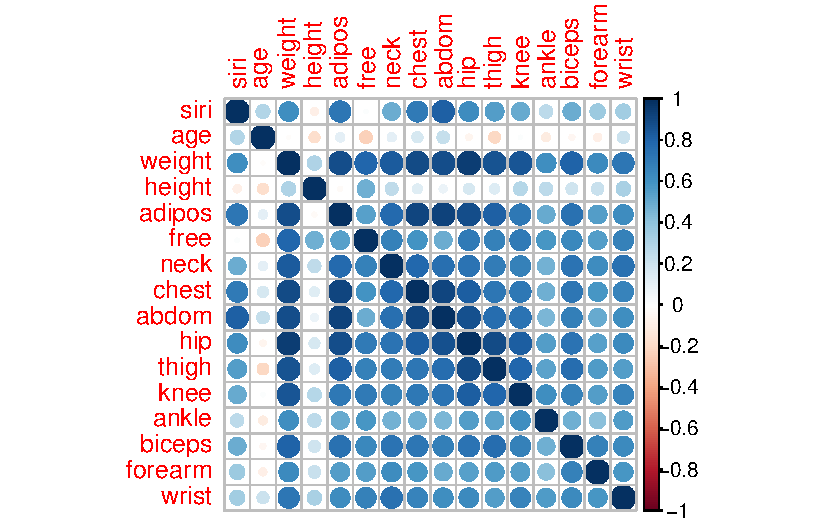
\includegraphics{Regularizacion_files/figure-pdf/unnamed-chunk-4-1.pdf}

}

\end{figure}

Podemos observar, como muchas de las variables estan íntimamente
correlacionadas, por lo tanto, a priori ya sabemos que nuestros modelos
múltiples lineales simples, no serán buenos.

Antes de empezar necesitamos escalar los datos

\begin{Shaded}
\begin{Highlighting}[]
\NormalTok{X }\OtherTok{\textless{}{-}} \FunctionTok{as.data.frame}\NormalTok{(}\FunctionTok{scale}\NormalTok{(X))}\DocumentationTok{\#\#para cada observación le va a quita la media para cada columna y la va a dividir entre la relación estandar de cada columna }
\end{Highlighting}
\end{Shaded}

\hypertarget{particiuxf3n-de-datos-prueba-y-entrenamiento}{%
\subsubsection{Partición de datos prueba y
entrenamiento}\label{particiuxf3n-de-datos-prueba-y-entrenamiento}}

\begin{Shaded}
\begin{Highlighting}[]
\NormalTok{train }\OtherTok{\textless{}{-}}\NormalTok{ X[}\SpecialCharTok{{-}}\FunctionTok{seq}\NormalTok{(}\DecValTok{10}\NormalTok{,}\DecValTok{252}\NormalTok{,}\DecValTok{10}\NormalTok{),]}
\NormalTok{test }\OtherTok{\textless{}{-}}\NormalTok{ X[}\FunctionTok{seq}\NormalTok{(}\DecValTok{10}\NormalTok{,}\DecValTok{252}\NormalTok{,}\DecValTok{10}\NormalTok{),]}
\end{Highlighting}
\end{Shaded}

\hypertarget{regresiuxf3n-lineal-muxfaltiple}{%
\subsubsection{Regresión lineal
múltiple}\label{regresiuxf3n-lineal-muxfaltiple}}

\begin{Shaded}
\begin{Highlighting}[]
\NormalTok{g  }\OtherTok{\textless{}{-}} \FunctionTok{lm}\NormalTok{(siri }\SpecialCharTok{\textasciitilde{}}\NormalTok{.,}\AttributeTok{data=}\NormalTok{train)}\DocumentationTok{\#\#Q1 es el 25\% de los datos{-}Q2 es el 75\% de los datos }
\FunctionTok{summary}\NormalTok{(g)}
\end{Highlighting}
\end{Shaded}

\begin{verbatim}

Call:
lm(formula = siri ~ ., data = train)

Residuals:
     Min       1Q   Median       3Q      Max 
-0.69681 -0.08032  0.02185  0.10933  0.79604 

Coefficients:
             Estimate Std. Error t value Pr(>|t|)    
(Intercept) -0.005917   0.012328  -0.480 0.631736    
age          0.012014   0.018553   0.648 0.517983    
weight       1.274772   0.081873  15.570  < 2e-16 ***
height       0.021458   0.017645   1.216 0.225315    
adipos      -0.224077   0.049727  -4.506 1.09e-05 ***
free        -1.230381   0.032435 -37.933  < 2e-16 ***
neck         0.004800   0.026103   0.184 0.854272    
chest        0.121106   0.039882   3.037 0.002694 ** 
abdom        0.180529   0.054356   3.321 0.001056 ** 
hip          0.005305   0.048026   0.110 0.912148    
thigh        0.122365   0.034165   3.582 0.000424 ***
knee         0.030732   0.026956   1.140 0.255542    
ankle        0.025340   0.016466   1.539 0.125325    
biceps       0.034730   0.023342   1.488 0.138278    
forearm      0.055722   0.017707   3.147 0.001888 ** 
wrist        0.015537   0.023070   0.673 0.501378    
---
Signif. codes:  0 '***' 0.001 '**' 0.01 '*' 0.05 '.' 0.1 ' ' 1

Residual standard error: 0.1852 on 211 degrees of freedom
Multiple R-squared:  0.9692,    Adjusted R-squared:  0.967 
F-statistic: 442.5 on 15 and 211 DF,  p-value: < 2.2e-16
\end{verbatim}

Observamos, cómo 7 variables son las más importantes en el modelo. De
hecho tenemos un R2 de casi el 97 porciento

\hypertarget{predicciuxf3n}{%
\paragraph{Predicción}\label{predicciuxf3n}}

\begin{Shaded}
\begin{Highlighting}[]
\NormalTok{predlm  }\OtherTok{\textless{}{-}} \FunctionTok{predict}\NormalTok{(g,test)}
\end{Highlighting}
\end{Shaded}

\hypertarget{regresiuxf3n-lineal-muxfaltiple.-selecciuxf3n-aic}{%
\subsubsection{Regresión lineal múltiple. Selección
AIC}\label{regresiuxf3n-lineal-muxfaltiple.-selecciuxf3n-aic}}

Lo podemos plantear manualmente

\begin{Shaded}
\begin{Highlighting}[]
\NormalTok{ conj }\OtherTok{\textless{}{-}} \FunctionTok{regsubsets}\NormalTok{(siri }\SpecialCharTok{\textasciitilde{}}\NormalTok{., }\AttributeTok{data=}\NormalTok{train, }\AttributeTok{nvmax =} \DecValTok{15}\NormalTok{)}
\NormalTok{ rconj }\OtherTok{\textless{}{-}} \FunctionTok{summary}\NormalTok{(conj)}
\NormalTok{ n }\OtherTok{\textless{}{-}} \FunctionTok{nrow}\NormalTok{(train)}
\NormalTok{ p }\OtherTok{\textless{}{-}} \FunctionTok{ncol}\NormalTok{(train[,}\SpecialCharTok{{-}}\DecValTok{1}\NormalTok{]) }\SpecialCharTok{+} \DecValTok{1}
\NormalTok{ aic }\OtherTok{\textless{}{-}}\NormalTok{ n}\SpecialCharTok{*}\FunctionTok{log}\NormalTok{(rconj}\SpecialCharTok{$}\NormalTok{rss}\SpecialCharTok{/}\NormalTok{n)}\SpecialCharTok{+}\NormalTok{(}\DecValTok{2}\SpecialCharTok{:}\NormalTok{p)}\SpecialCharTok{*}\DecValTok{2}
 \FunctionTok{plot}\NormalTok{(}\DecValTok{1}\SpecialCharTok{:}\NormalTok{(p}\DecValTok{{-}1}\NormalTok{),aic,}\AttributeTok{ylab=}\StringTok{"AIC"}\NormalTok{,}\AttributeTok{xlab=}\StringTok{"Número de predictores"}\NormalTok{,}\AttributeTok{axes=}\NormalTok{F)}
 \FunctionTok{box}\NormalTok{(); }\FunctionTok{axis}\NormalTok{(}\DecValTok{1}\NormalTok{,}\AttributeTok{at=}\DecValTok{1}\SpecialCharTok{:}\NormalTok{(p}\DecValTok{{-}1}\NormalTok{)); }\FunctionTok{axis}\NormalTok{(}\DecValTok{2}\NormalTok{)}
\end{Highlighting}
\end{Shaded}

\begin{figure}[H]

{\centering 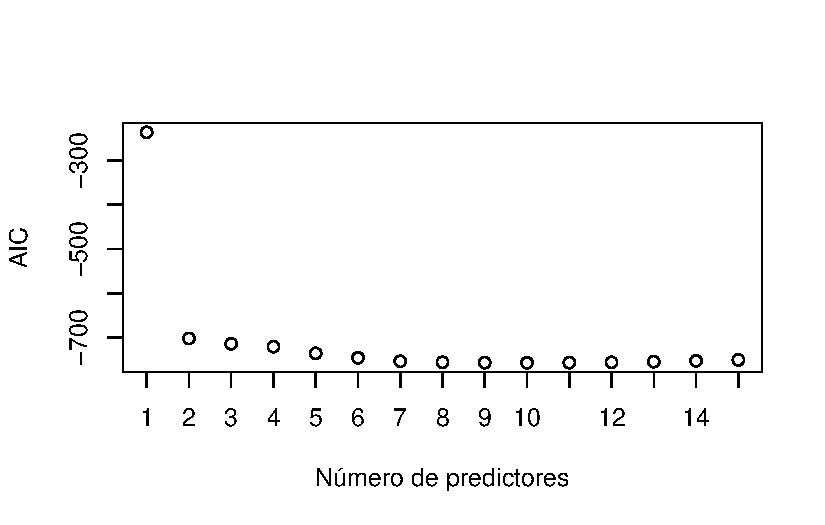
\includegraphics{Regularizacion_files/figure-pdf/unnamed-chunk-9-1.pdf}

}

\end{figure}

El mínimo AIC se obtiene con

\begin{Shaded}
\begin{Highlighting}[]
\FunctionTok{which.min}\NormalTok{(aic)}
\end{Highlighting}
\end{Shaded}

\begin{verbatim}
[1] 10
\end{verbatim}

pero con 7, 8 o 9 predictoras, el valor de AIC es similar.

Si se utiliza la función \texttt{step()}, se minimiza el AIC con un
modelo de 10 predictores

\begin{Shaded}
\begin{Highlighting}[]
\NormalTok{lmaic }\OtherTok{\textless{}{-}} \FunctionTok{step}\NormalTok{(g, }\AttributeTok{trace =}\NormalTok{ F)}\DocumentationTok{\#\#step hace cada combinación posible de las variables hasta que tenga el mejor modelo }
\FunctionTok{formula}\NormalTok{(lmaic)}
\end{Highlighting}
\end{Shaded}

\begin{verbatim}
siri ~ weight + adipos + free + chest + abdom + thigh + knee + 
    ankle + biceps + forearm
\end{verbatim}

\begin{Shaded}
\begin{Highlighting}[]
\NormalTok{predaic }\OtherTok{\textless{}{-}} \FunctionTok{predict}\NormalTok{(lmaic,test)}
\end{Highlighting}
\end{Shaded}

\hypertarget{pcr}{%
\subsubsection{PCR}\label{pcr}}

\begin{Shaded}
\begin{Highlighting}[]
\NormalTok{mpc }\OtherTok{\textless{}{-}} \FunctionTok{pcr}\NormalTok{(siri }\SpecialCharTok{\textasciitilde{}}\NormalTok{., }\AttributeTok{data=}\NormalTok{train, }\AttributeTok{validation=}\StringTok{"CV"}\NormalTok{)}
\NormalTok{mpcCV }\OtherTok{\textless{}{-}} \FunctionTok{RMSEP}\NormalTok{(mpc, }\AttributeTok{estimate=}\StringTok{"CV"}\NormalTok{)}
\NormalTok{(numpredcp }\OtherTok{\textless{}{-}} \FunctionTok{which.min}\NormalTok{(mpcCV}\SpecialCharTok{$}\NormalTok{val))}
\end{Highlighting}
\end{Shaded}

\begin{verbatim}
[1] 12
\end{verbatim}

En este caso el número de predictores seleccionados es de 7 (descontando
el intercept).

\begin{Shaded}
\begin{Highlighting}[]
\NormalTok{predcp }\OtherTok{\textless{}{-}} \FunctionTok{predict}\NormalTok{(mpc, test, }\AttributeTok{ncomp=}\NormalTok{numpredcp}\DecValTok{{-}1}\NormalTok{)}
\end{Highlighting}
\end{Shaded}

\hypertarget{regresion-por-muxednimos-cuadrados-parciales-pls}{%
\subsubsection{Regresion por mínimos cuadrados parciales
(PLS)}\label{regresion-por-muxednimos-cuadrados-parciales-pls}}

\begin{Shaded}
\begin{Highlighting}[]
\FunctionTok{set.seed}\NormalTok{(}\DecValTok{123456}\NormalTok{)}
\NormalTok{mpls }\OtherTok{\textless{}{-}} \FunctionTok{plsr}\NormalTok{(siri}\SpecialCharTok{\textasciitilde{}}\NormalTok{., }\AttributeTok{data=}\NormalTok{train, }\AttributeTok{validation=}\StringTok{"CV"}\NormalTok{)}
\NormalTok{mplsCV }\OtherTok{\textless{}{-}} \FunctionTok{RMSEP}\NormalTok{(mpls, }\AttributeTok{estimate=}\StringTok{"CV"}\NormalTok{)}
\NormalTok{(numpredpls}\OtherTok{\textless{}{-}}\FunctionTok{which.min}\NormalTok{(mplsCV}\SpecialCharTok{$}\NormalTok{val) }\SpecialCharTok{{-}} \DecValTok{1}\NormalTok{)}
\end{Highlighting}
\end{Shaded}

\begin{verbatim}
[1] 4
\end{verbatim}

\begin{Shaded}
\begin{Highlighting}[]
\NormalTok{predpls }\OtherTok{\textless{}{-}} \FunctionTok{predict}\NormalTok{(mpls,test,}\AttributeTok{ncomp=}\NormalTok{numpredpls)}
\end{Highlighting}
\end{Shaded}

\hypertarget{regresiuxf3n-contrauxedda-ridge}{%
\subsubsection{Regresión contraída
(RIDGE)}\label{regresiuxf3n-contrauxedda-ridge}}

\begin{Shaded}
\begin{Highlighting}[]
\NormalTok{mr }\OtherTok{\textless{}{-}} \FunctionTok{lm.ridge}\NormalTok{(siri }\SpecialCharTok{\textasciitilde{}}\NormalTok{., }\AttributeTok{data=}\NormalTok{datos, }\AttributeTok{lambda=}\NormalTok{(}\FunctionTok{seq}\NormalTok{(}\DecValTok{0}\NormalTok{,}\FloatTok{0.01}\NormalTok{,}\FloatTok{0.0001}\NormalTok{)))}
\NormalTok{(nGCV }\OtherTok{\textless{}{-}} \FunctionTok{which.min}\NormalTok{(mr}\SpecialCharTok{$}\NormalTok{GCV))}
\end{Highlighting}
\end{Shaded}

\begin{verbatim}
0.0024 
    25 
\end{verbatim}

\begin{Shaded}
\begin{Highlighting}[]
\FunctionTok{set.seed}\NormalTok{(}\DecValTok{124568919}\NormalTok{)}
\NormalTok{lGCV }\OtherTok{\textless{}{-}}\NormalTok{ mr}\SpecialCharTok{$}\NormalTok{lambda[nGCV]}
\FunctionTok{matplot}\NormalTok{(mr}\SpecialCharTok{$}\NormalTok{lambda,}\FunctionTok{coef}\NormalTok{(mr),}\AttributeTok{type=}\StringTok{"l"}\NormalTok{, }\AttributeTok{ylim=}\FunctionTok{c}\NormalTok{(}\SpecialCharTok{{-}}\DecValTok{2}\NormalTok{,}\DecValTok{2}\NormalTok{),                 }\AttributeTok{xlab=}\FunctionTok{expression}\NormalTok{(lambda),}\AttributeTok{ylab=}\FunctionTok{expression}\NormalTok{(hatbeta[i]))}
\FunctionTok{abline}\NormalTok{(}\AttributeTok{v=}\NormalTok{lGCV,}\AttributeTok{col=}\DecValTok{2}\NormalTok{)}
\end{Highlighting}
\end{Shaded}

\begin{figure}[H]

{\centering 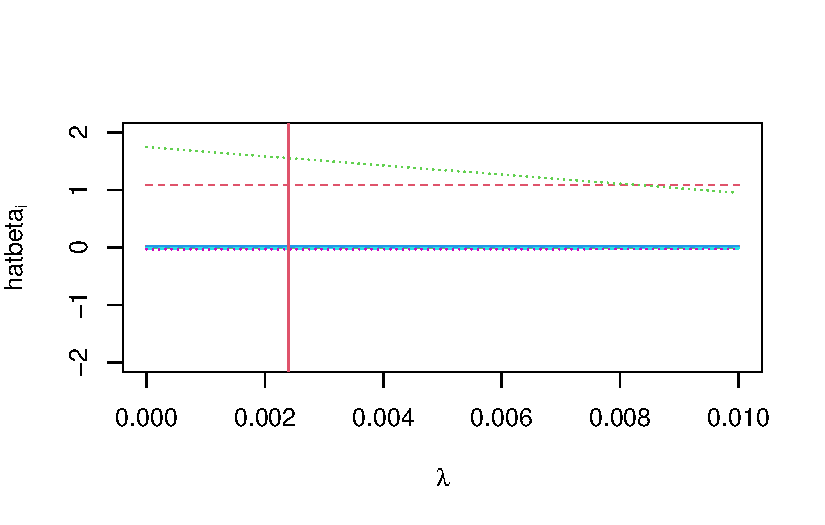
\includegraphics{Regularizacion_files/figure-pdf/unnamed-chunk-16-1.pdf}

}

\end{figure}

\begin{Shaded}
\begin{Highlighting}[]
\FunctionTok{plot}\NormalTok{(mr}\SpecialCharTok{$}\NormalTok{lambda,mr}\SpecialCharTok{$}\NormalTok{GCV,}\AttributeTok{type=}\StringTok{"l"}\NormalTok{,}\AttributeTok{xlab=}\FunctionTok{expression}\NormalTok{(lambda),}\AttributeTok{ylab=}\StringTok{"GCV"}\NormalTok{)}
\FunctionTok{abline}\NormalTok{(}\AttributeTok{v=}\NormalTok{lGCV,}\AttributeTok{col=}\DecValTok{2}\NormalTok{)}
\end{Highlighting}
\end{Shaded}

\begin{figure}[H]

{\centering 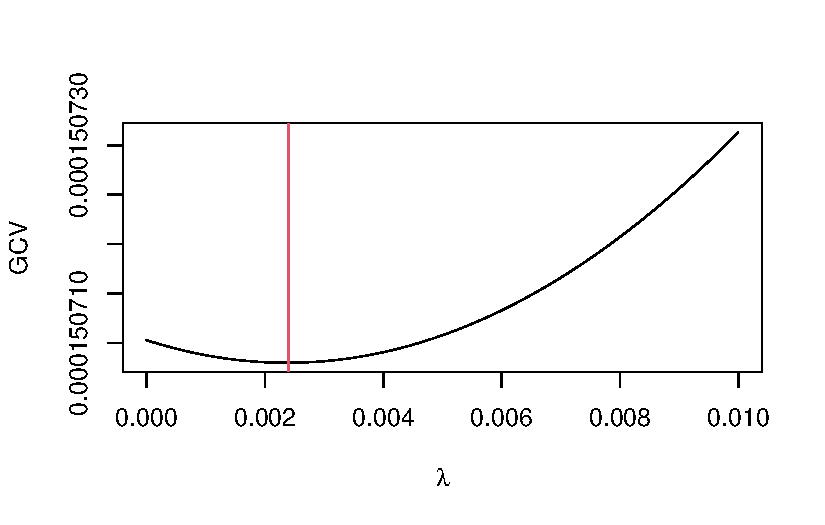
\includegraphics{Regularizacion_files/figure-pdf/unnamed-chunk-17-1.pdf}

}

\end{figure}

\begin{Shaded}
\begin{Highlighting}[]
\NormalTok{ mr }\OtherTok{\textless{}{-}} \FunctionTok{lm.ridge}\NormalTok{(siri}\SpecialCharTok{\textasciitilde{}}\NormalTok{.,train, }\AttributeTok{lambda=}\NormalTok{lGCV)}
\NormalTok{ predridge }\OtherTok{\textless{}{-}} \FunctionTok{cbind}\NormalTok{(}\DecValTok{1}\NormalTok{,}\FunctionTok{as.matrix}\NormalTok{(test[,}\SpecialCharTok{{-}}\DecValTok{1}\NormalTok{])) }\SpecialCharTok{\%*\%} \FunctionTok{coef}\NormalTok{(mr)}
\end{Highlighting}
\end{Shaded}

\hypertarget{regresiuxf3n-lasso}{%
\subsubsection{Regresión LASSO}\label{regresiuxf3n-lasso}}

\begin{Shaded}
\begin{Highlighting}[]
\CommentTok{\#perform k{-}fold cross{-}validation to find optimal lambda value}
\NormalTok{train.matrix }\OtherTok{\textless{}{-}} \FunctionTok{as.matrix}\NormalTok{(train)}
\NormalTok{X }\OtherTok{\textless{}{-}}\NormalTok{ train.matrix[,}\SpecialCharTok{{-}}\DecValTok{1}\NormalTok{]}
\NormalTok{y }\OtherTok{\textless{}{-}}\NormalTok{ train.matrix[,}\DecValTok{1}\NormalTok{]}
\NormalTok{mod\_cv }\OtherTok{\textless{}{-}} \FunctionTok{cv.glmnet}\NormalTok{(}\AttributeTok{x=}\NormalTok{X, }\AttributeTok{y=}\NormalTok{y, }\AttributeTok{family=}\StringTok{"gaussian"}\NormalTok{,}
                        \AttributeTok{intercept =}\NormalTok{ F, }\AttributeTok{alpha=}\DecValTok{1}\NormalTok{)}
\CommentTok{\#find optimal lambda value that minimizes test MSE}
\NormalTok{best\_lambda }\OtherTok{\textless{}{-}}\NormalTok{ mod\_cv}\SpecialCharTok{$}\NormalTok{lambda.min}
\NormalTok{best\_lambda}
\end{Highlighting}
\end{Shaded}

\begin{verbatim}
[1] 0.01666548
\end{verbatim}

\begin{Shaded}
\begin{Highlighting}[]
\CommentTok{\#produce plot of test MSE by lambda value}
\FunctionTok{plot}\NormalTok{(mod\_cv) }
\end{Highlighting}
\end{Shaded}

\begin{figure}[H]

{\centering 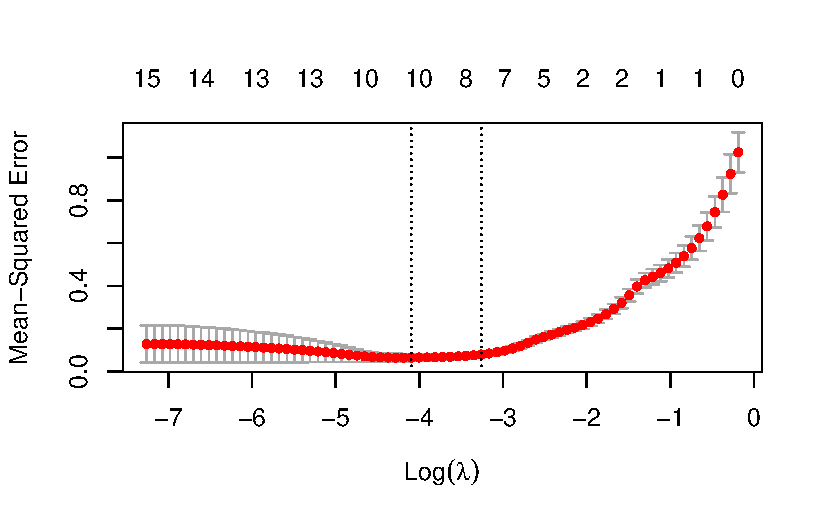
\includegraphics{Regularizacion_files/figure-pdf/unnamed-chunk-19-1.pdf}

}

\end{figure}

\begin{Shaded}
\begin{Highlighting}[]
\NormalTok{test.matrix }\OtherTok{\textless{}{-}} \FunctionTok{as.matrix}\NormalTok{(test)}
\NormalTok{predlasso }\OtherTok{\textless{}{-}} \FunctionTok{predict}\NormalTok{(mod\_cv,test.matrix[,}\SpecialCharTok{{-}}\DecValTok{1}\NormalTok{])}
\end{Highlighting}
\end{Shaded}

\hypertarget{resumen}{%
\subsection{Resumen}\label{resumen}}

\begin{Shaded}
\begin{Highlighting}[]
\NormalTok{ rmse }\OtherTok{\textless{}{-}} \ControlFlowTok{function}\NormalTok{(x,y) }\FunctionTok{sqrt}\NormalTok{(}\FunctionTok{mean}\NormalTok{((x}\SpecialCharTok{{-}}\NormalTok{y)}\SpecialCharTok{\^{}}\DecValTok{2}\NormalTok{))}
\NormalTok{ rmse.lm }\OtherTok{\textless{}{-}} \FunctionTok{rmse}\NormalTok{(predlm,test}\SpecialCharTok{$}\NormalTok{siri)}
\NormalTok{ rmse.aic }\OtherTok{\textless{}{-}} \FunctionTok{rmse}\NormalTok{(predaic,test}\SpecialCharTok{$}\NormalTok{siri)}
\NormalTok{ rmse.cp }\OtherTok{\textless{}{-}} \FunctionTok{rmse}\NormalTok{(predcp,test}\SpecialCharTok{$}\NormalTok{siri)}
\NormalTok{ rmse.pls }\OtherTok{\textless{}{-}} \FunctionTok{rmse}\NormalTok{(predpls,test}\SpecialCharTok{$}\NormalTok{siri)}
\NormalTok{ rmse.ridge }\OtherTok{\textless{}{-}} \FunctionTok{rmse}\NormalTok{(predridge,test}\SpecialCharTok{$}\NormalTok{siri)}
\NormalTok{ rmse.lasso }\OtherTok{\textless{}{-}} \FunctionTok{rmse}\NormalTok{(predlasso,test}\SpecialCharTok{$}\NormalTok{siri)}
 
\NormalTok{ res }\OtherTok{\textless{}{-}} \FunctionTok{data.frame}\NormalTok{(}\AttributeTok{lm=}\NormalTok{rmse.lm,}
            \AttributeTok{aic=}\NormalTok{rmse.aic,}
            \AttributeTok{pcr =}\NormalTok{ rmse.cp,}
            \AttributeTok{pls =}\NormalTok{ rmse.pls,}
            \AttributeTok{ridge=}\NormalTok{rmse.ridge,}
            \AttributeTok{lasso=}\NormalTok{rmse.lasso)}
 
\NormalTok{ res }\OtherTok{\textless{}{-}} \FunctionTok{as.data.frame}\NormalTok{(}\FunctionTok{t}\NormalTok{(}\FunctionTok{round}\NormalTok{(res,}\DecValTok{4}\NormalTok{)))}
\NormalTok{res}
\end{Highlighting}
\end{Shaded}

\begin{verbatim}
          V1
lm    0.1352
aic   0.1341
pcr   0.1999
pls   0.2012
ridge 0.1352
lasso 0.2015
\end{verbatim}



\end{document}
